\documentclass[11pt]{article}
\usepackage[latin1]{inputenc}
\usepackage{amsmath}
\usepackage{amsfonts}
\usepackage{amssymb}
\usepackage{xcolor}
\usepackage{makeidx}
\usepackage{graphicx, array}
\usepackage{pgf,tikz}
\usepackage{tkz-euclide}
\usepackage{pgfplots}
\pgfplotsset{compat=1.9}
\usetkzobj{all}
\pagestyle{empty}
\usepackage{enumerate}
\usepackage[margin = 0.5in]{geometry}
\pagestyle{empty}
\raggedright

\begin{document}

Name \makebox[2.5in]{\hrulefill}    \hfill  Honors PreCalc P-set

\subsubsection*{Function Operations \hfill \makebox[0.35in]{\hrulefill} / 10}

Simplify or evaluate each for $f(x) = 3x + 7$, $g(x) = -2x^2 - 1$, $h(x) = \sqrt{x + 1}$, and $j(x) = x^3$.
\begin{flalign*}
1.  \quad   &   (f + g)(1)          &
2.  \quad   &   (h - f)(3)          &
3.  \quad   &   (f \cdot j)(-2)     &&\\[1in]
4.  \quad   &   (f - g)(x)          &
5.  \quad   &   (f \cdot g)(x)      &
6.  \quad   &   (h \cdot h)(x)      &&\\[1.25in]
7.  \quad   &   \left(\frac{g}{j}\right)(x)      &
8.  \quad   &   \left(\frac{f}{j}\right)(3) &
9.  \quad   &   (h \cdot j)(2)             &&\\[1.25in]
10. \quad   &   (f + g)(x)             &
11. \quad   &   (j \cdot g)(x)      &
12. \quad   &   g(2) - h(15)        &&\\[1.25in]
\end{flalign*}
\smallskip

Find the difference quotient for each.
\begin{flalign*}
13. \quad   &   f(x) = 6x + 7   &
14. \quad   &   f(x) = x^2 - 9  &
15. \quad   &   f(x) = 5x^2 - 3x + 4    &&\\
\end{flalign*}

\newpage

Use the graph to evaluate each.
\newline\\

\begin{center}

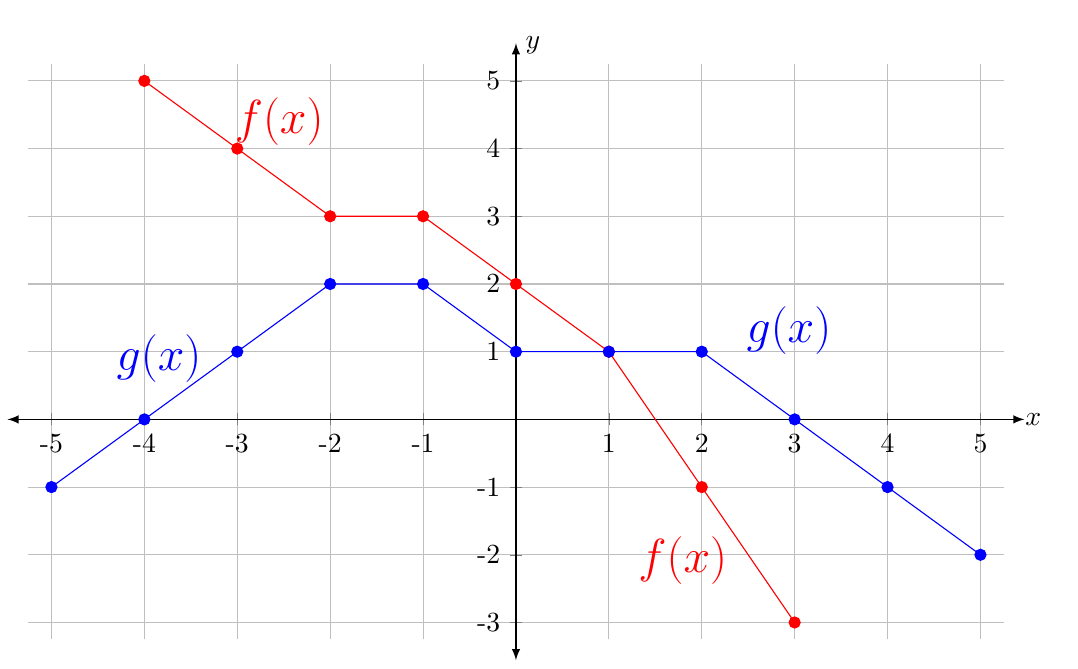
\begin{tikzpicture}

\begin{axis}
[   
    grid,
    axis lines=middle,
    xmin=-5.25,xmax=5.25,
    ymin=-3.25,ymax=5.25,
    restrict y to domain=-3:5,
    xtick={-5,-4,...,5},
    xticklabels={-5,-4,-3,-2,-1,,1,2,3,4,5},
    ytick={-3,-2,...,5},
    yticklabels={-3,-2,-1,,1,2,3,4,5},
    axis line style={latex-latex},
    axis line style={shorten >=-7.5pt, shorten <=-7.5pt},
    xlabel=$x$,
    ylabel=$y$,
    xlabel style={at={(ticklabel* cs:1)},anchor=west, xshift=0.15cm},
    ylabel style={at={(ticklabel* cs:1)},anchor=south west},
    width=5.5in,
    height=3.5in
]
\addplot[mark = *, color=red] coordinates
{
    (-4,5)
    (-3,4)
    (-2,3)
    (-1,3)
    (0,2)
    (1,1)
    (2,-1)
    (3,-3)
};
\addplot[mark=*, color=blue] coordinates
{
    (-5,-1)
    (-4,0)  
    (-3,1)
    (-2,2)
    (-1,2)
    (0,1)
    (1,1)
    (2,1)
    (3,0)
    (4,-1)
    (5,-2)
};
\end{axis}
\node at (2.5,7) [anchor = north west] {\color{red}\LARGE $f(x)$};
\node at (9,1) [anchor = east] {\color{red}\LARGE $f(x)$};
\node at (1,4) [anchor = north west] {\color{blue} \LARGE $g(x)$};
\node at (9,3.5) [anchor = south west] {\color{blue} \LARGE $g(x)$};
\end{tikzpicture}
\end{center}

\begin{flalign*}
16. \quad   &   f(2) + g(4)         &
17. \quad   &   g(-1) \cdot g(-3)   &
18. \quad   &   (f - g)(2)      &
19. \quad   &   \left(\frac{g}{f}\right)(-2)            &&\\[1in]
\end{flalign*}

\fbox{\emph{Level 2}}
\newline\\

20. A balloon is is being filled with air. The radius $r$ is increasing with time $t$ (in seconds) according to the formula $r(t) = \frac{1}{2}t^2$. \newline\\
Using the volume formula for a sphere, $V(r) = \frac{4}{3}\pi r ^3$, find the volume as a function of time.
\\[1.5in]


21. If $f$ and $g$ are odd functions, show that $f \circ g$ is also odd.



\newpage


\textbf{Function Operations and Compositions KEY}

\begin{enumerate}
    \item 7
    \item $-14$
    \item $-8$
    \item $2x^2+3x+8$
    \item $-6x^3-14x^2-3x-7$
    \item $x+1$
    \item $\frac{-2x^2-1}{x^3}$, or $\frac{-2}{x}-\frac{1}{x^3}$
    \item $\frac{16}{27}$
    \item $8\sqrt{2}$
    \item $-2x^2+3x+6$
    \item $-2x^5-x^3$
    \item $-13$
    \item 6
    \item $2x+h$
    \item $10x + 5h - 3$
    \item $-2$
    \item 2
    \item $-2$
    \item $\frac{2}{3}$
\end{enumerate}



\end{document}
